Did you know that a typical organization loses 5\% of its revenue to fraud each year? In fact, it is estimated that fraud is costing the UK economy 73 billion British pounds each year. As such, you can say, fraud poses a serious problem to almost all companies. This course teaches you how you can tackle fraud as a data scientist, and thereby make a tangible impact on your company.

\subsection{What is fraud?}

Fraudulent behavior can be found in many different areas. Credit card fraud is perhaps the most famous example, and also in the insurance industry, fraud is a well-known issue. But it is much more broadly present than that. For example even all e-commerce businesses need to continuously assess whether client transactions on their website are legit. Detecting fraud is typically challenging because of these four characteristics of fraud described here. First of all, fraud cases are in a minority, sometimes only one-hundredth percent of a companies' transactions are fraudulent. Fraudsters will also try their best to "blend" in and conceal their activities. Moreover, fraudsters will find new methods to avoid getting caught, and change their behavior over time. Lastly, fraudsters oftentimes work together and organize their activities in a network, making it harder to detect. It can be that multiple client accounts are involved around one fraud case. Let's illustrate this with an example.

\subsection{Fraud detection is challenging}
Have you ever played "Where is Waldo" or "Find the odd one out"? Like in the game, in fraud detection you'll need to train an algorithm to pick a well concealed observation out of many normal observations. It looks like the other clovers, but it deviates slightly as it has 3 leafs instead of four. That one was easy, but it does get much harder when we're working with numbers. This is much more like in real life, we'll need to find a fraud case based on numbers. This illustrates a typical fraud detection problem really well: based on data, you'll need to train an algorithm to find the odd one out among many normal observations.

\subsection{How companies deal with fraud}

As a data scientist working on fraud analytics, you'll often be asked to improve existing fraud detection systems. You'll maybe find that the company already uses a rules based system to filter out strange cases. Or that the fraud analytics team checks the news for suspicious names, or keeps track of external hit lists from the police to reference check against the client base. All these existing methods can be useful for your machine learning model, as you can use them as inputs in your analysis. But do be mindful when using labels that come out of existing rules based systems; you should always ask yourself whether the labels are reliable as they might not catch all fraudulent cases.

\subsection{Let's have a look at some data}
In this chapter we'll explore a dataset on credit card transactions. We have 29 features available, and a \lstinline!Class! variable, containing information about whether the transaction is fraudulent or not. We have data on 5050 transactions in total. This should be enough for training our first algorithm on. Now let's have a look at this credit card data in more detail!

\subsection{Checking the fraud to non-fraud ratio}
In this chapter, you will work on \lstinline!creditcard_sampledata_3.csv!, a dataset containing credit card transactions data. Fraud occurrences are fortunately an \textbf{extreme minority} in these transactions.

However, Machine Learning algorithms usually work best when the different classes contained in the dataset are more or less equally present. If there are few cases of fraud, then there's little data to learn how to identify them. This is known as \textbf{class imbalance}, and it's one of the main challenges of fraud detection.

Let's explore this dataset, and observe this class imbalance problem.

\begin{lstlisting}[language={python}]
import pandas as pd
import config

df = pd.read_csv(config.DATAPATH / "chapter_1/creditcard_sampledata.csv")
print(df.head())
\end{lstlisting}

\begin{lstlisting}[language={bash}]
   Unnamed: 0  Time        V1        V2  ...       V27       V28  Amount  Class
0           0    64  1.212511 -0.099054  ...  0.020370  0.017037   34.70      0
1           1    64 -0.658305  0.406791  ... -0.094192 -0.092493   54.99      0
2           2   124  1.105253  0.541842  ...  0.000208  0.026167    6.24      0
3           3   128  1.239495 -0.182609  ...  0.036867  0.010963    8.80      0
4           4   132 -1.571359  1.687508  ... -0.481570 -0.167897   10.00      0
[5 rows x 32 columns]
\end{lstlisting}

\begin{lstlisting}[language={python}]
df.info()
\end{lstlisting}

\begin{lstlisting}[language={bash}]
<class 'pandas.core.frame.DataFrame'>
RangeIndex: 8000 entries, 0 to 7999
Data columns (total 32 columns):
 #   Column      Non-Null Count  Dtype  
---  ------      --------------  -----  
 0   Unnamed: 0  8000 non-null   int64  
 1   Time        8000 non-null   int64  
 2   V1          8000 non-null   float64
 3   V2          8000 non-null   float64
 4   V3          8000 non-null   float64
 5   V4          8000 non-null   float64
 6   V5          8000 non-null   float64
 7   V6          8000 non-null   float64
 8   V7          8000 non-null   float64
 9   V8          8000 non-null   float64
 10  V9          8000 non-null   float64
 11  V10         8000 non-null   float64
 12  V11         8000 non-null   float64
 13  V12         8000 non-null   float64
 14  V13         8000 non-null   float64
 15  V14         8000 non-null   float64
 16  V15         8000 non-null   float64
 17  V16         8000 non-null   float64
 18  V17         8000 non-null   float64
 19  V18         8000 non-null   float64
 20  V19         8000 non-null   float64
 21  V20         8000 non-null   float64
 22  V21         8000 non-null   float64
 23  V22         8000 non-null   float64
 24  V23         8000 non-null   float64
 25  V24         8000 non-null   float64
 26  V25         8000 non-null   float64
 27  V26         8000 non-null   float64
 28  V27         8000 non-null   float64
 29  V28         8000 non-null   float64
 30  Amount      8000 non-null   float64
 31  Class       8000 non-null   int64  
dtypes: float64(29), int64(3)
memory usage: 2.0 MB
\end{lstlisting}

\begin{lstlisting}[language={python}]
# Count the occurrences of fraud and no fraud and print them
occ = df['Class'].value_counts()
print(occ)
\end{lstlisting}

\begin{lstlisting}[language={bash}]
0    7983
1      17
Name: Class, dtype: int64
\end{lstlisting}

\begin{lstlisting}[language={python}]
# Print the ratio of fraud cases
print(occ / len(df))
\end{lstlisting}

\begin{lstlisting}[language={bash}]
0    0.997875
1    0.002125
Name: Class, dtype: float64
\end{lstlisting}

As you can see, the ratio of fraudulent transactions is very low. This is a case of class imbalance problem, and you're going to learn how to deal with this in the next exercises.

\subsection{Plotting our data}

From the previous exercise we know that the ratio of fraud to non-fraud observations is very low. You can do something about that, for example by \textbf{re-sampling} our data, which is explained in the next video.

In this exercise, you'll look at the data and \textbf{visualize the fraud to non-fraud ratio}. It is always a good starting point in your fraud analysis, to look at your data first, before you make any changes to it.

Moreover, when talking to your colleagues, a picture often makes it very clear that we're dealing with heavily imbalanced data. Let's create a plot to visualize the ratio fraud to non-fraud data points on the dataset \lstinline!df!.

\begin{lstlisting}[language={python}]
import matplotlib.pyplot as plt
import numpy as np


def prep_data(df):
    X = df.iloc[:, 1:29]
    X = np.array(X).astype(float)
    y = df.iloc[:, 29]
    y=np.array(y).astype(float)
    return X, y


# Define a function to create a scatter plot of our data and labels
def plot_data(X, y):
    plt.scatter(X[y == 0, 0], X[y == 0, 1], label="Class #0", alpha=0.5, linewidth=0.15)
    plt.scatter(X[y == 1, 0], X[y == 1, 1], label="Class #1", alpha=0.5, linewidth=0.15, c='r')
    plt.legend()
    return plt.show()
\end{lstlisting}

By visualizing your data you can immediately see how our fraud cases are scattered over our data, and how few are cases we have. A picture often makes the imbalance problem often very clear. In the next exercises we'll visually explore how to improve our fraud to non-fraud balance.

\begin{figure}
	\centering
	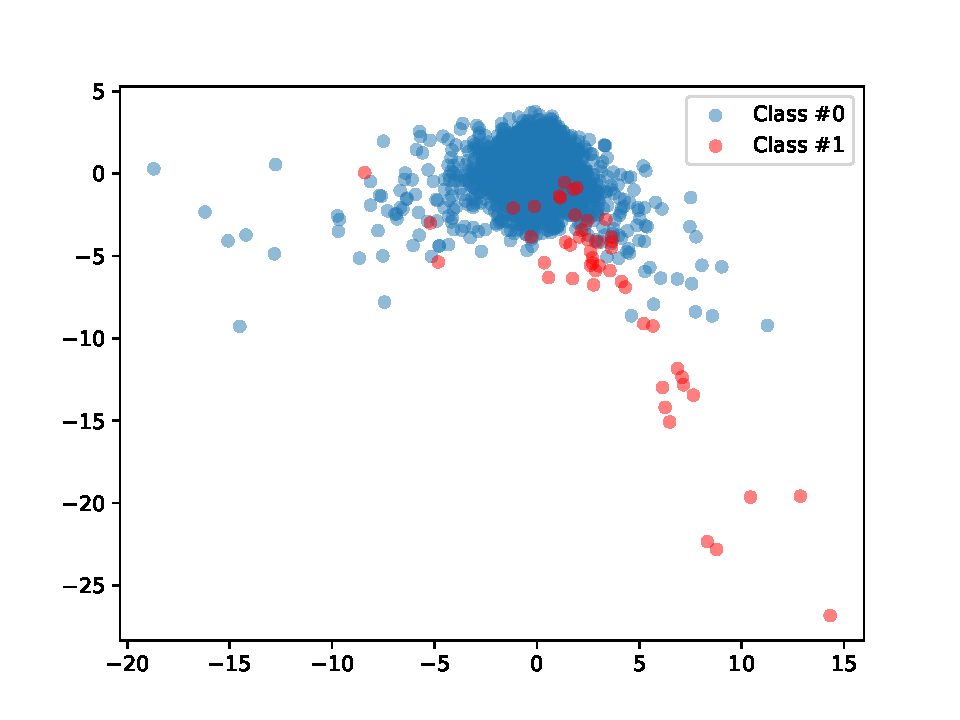
\includegraphics[width=0.5\textwidth]{plots/data.pdf}
\end{figure}




